\subsection{MetaNetwork}
By clicking toolsets and then MetaNetwork,
users are directed to MetaNetwork home page as Figure~\ref{fig:MetaNetworkHome}.
The R package for MetaNetwork module can be found \url{https://github.com/metaOmics/MetaNetwork}.

\begin{figure}[H]
\begin{center}
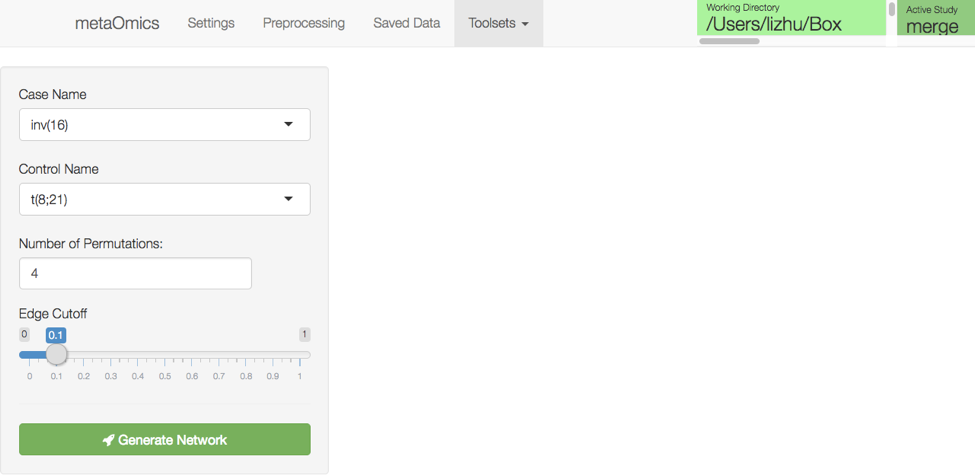
\includegraphics[scale=0.5]{./figure/MetaNetwork/MetaNetworkHome}
\caption{MetaNetwork homepage}
\label{fig:MetaNetworkHome}
\end{center}
\end{figure}

MetaNetwork includes three steps to get differentially co-expressed networks,
including (1) generate network, (2) search for basic modules, and (3) assemble super-modules. 
The left side of Figure~\ref{fig:MetaNetworkHome} is the control panel of step 1. 
The control panel for step 2 and step 3 will show up after the previous step is done.
The explanation of the complete list of all options are in Section~\ref{sec:completeList_MetaNetwork}


\subsubsection{Procedure}

\begin{steps}
\item \textbf{Generate Network}
The first step of MetaNetwork is to generate co-expression network. 
In this step, the network for permuted data will also be generated. 
Users need to select case and control names, the number of permutations, and edge cut-off which determines the proportion of edges to be kept in the network. 
After clicking \textbf{Generate Network} button, screen will show message indicating the algorithm is running to generate network.

\item \textbf{Search for basic modules}

The next step is to search basic modules.
Advanced options (recommended not to change) include the number of repeats used for each initial seed modules (``Number of repeat"),
the maximim Monte Carlo steps for simulated annealing algorithm (MC Steps),
and the maximum pairwise Jaccard index allowed for basic modules (Jaccard Cutoff), as shown in Figure~\ref{fig:MetaNetworkstep2}.
Explanation of these technical terms are omitted in this tutorial,
but readers can refer to \cite{zhu2016metadcn} for details.
After clicking \textbf{Search for basic modules} button in Figure~\ref{fig:MetaNetworkstep2}, 
screen will show message indicating the algorithm is running to search for basic modules.
This step is computationally demanding depending the on gene size.
After this step is done,
the screen will show a table of basic modules highly connected in cases but lose connections in control and vice versa.


\begin{figure}[H]
\begin{center}
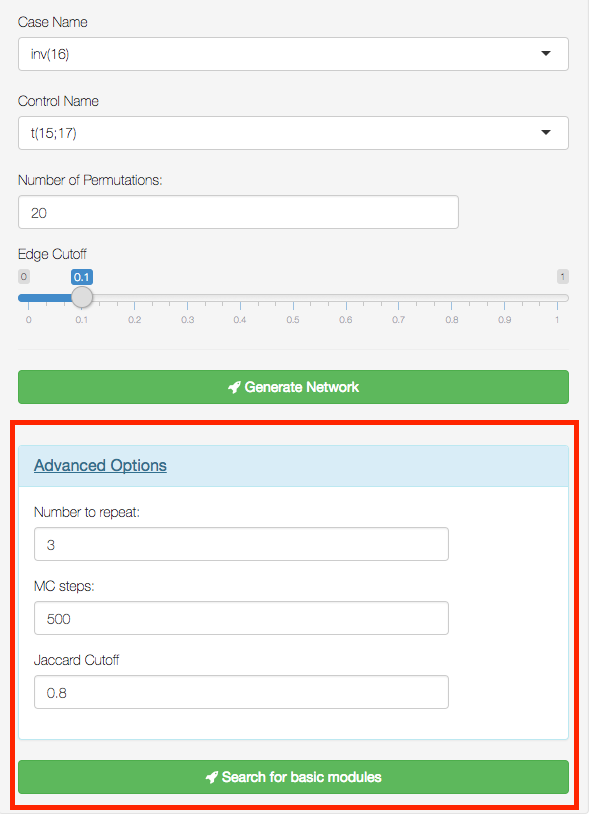
\includegraphics[scale=0.35]{./figure/MetaNetwork/MetaNetworkstep2}
\caption{MetaNetwork control panel for search for basic modules}
\label{fig:MetaNetworkstep2}
\end{center}
\end{figure}

Search for basic modules can be time consuming, 
especially if a large number of genes are used. 
After this step is done, the screen will show a table of basic modules higher correlated in case and a table of basic modules higher correlated in control as in Figure~\ref{fig:MetaNetworkBM}. 

\begin{figure}[H]
\begin{center}
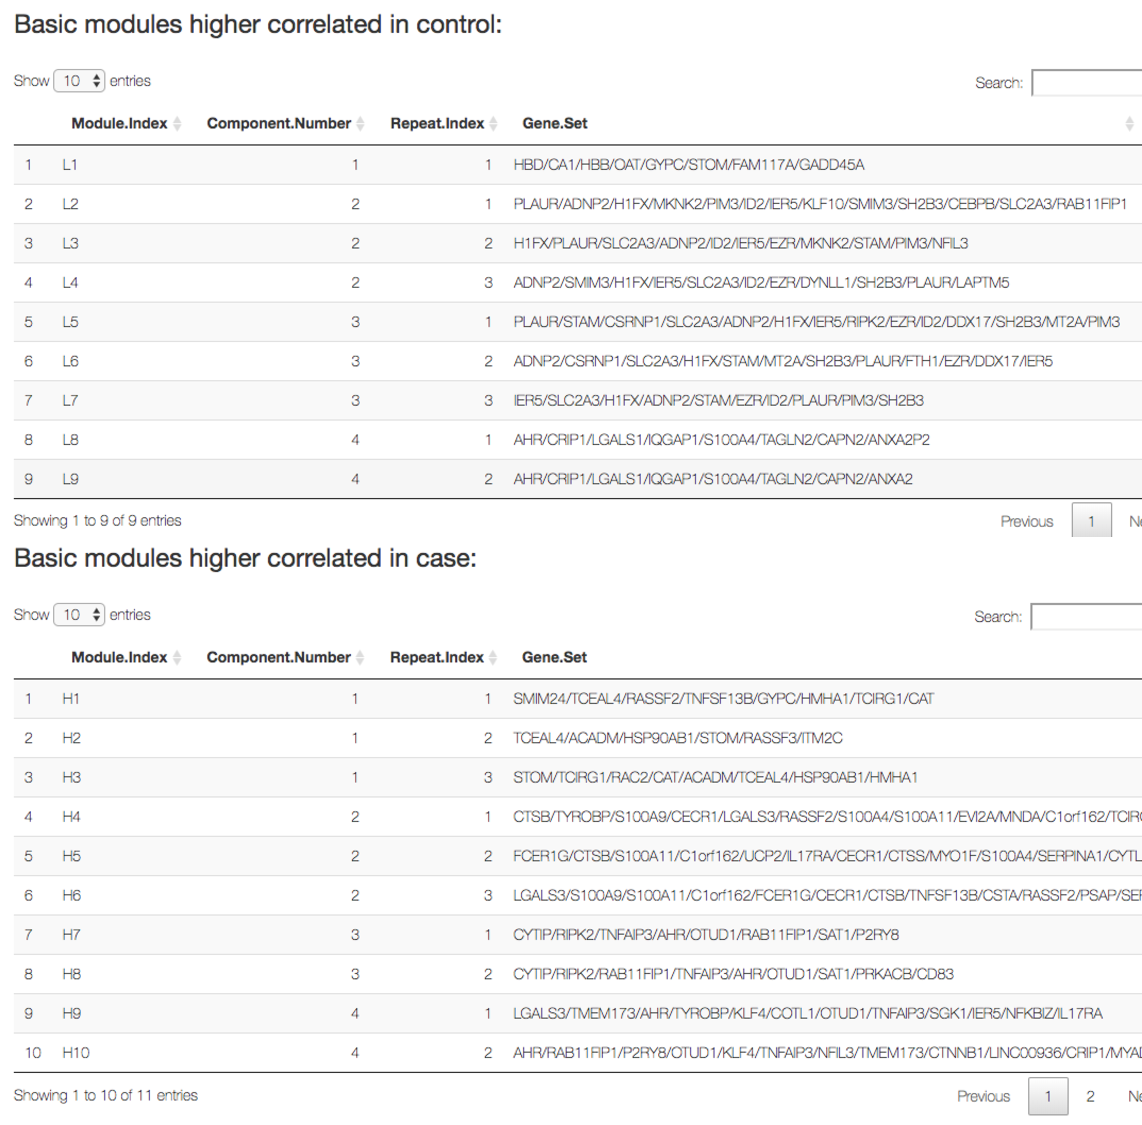
\includegraphics[scale=0.9]{./figure/MetaNetwork/MetaNetworkBM}
\caption{MetaNetwork output from search for basic modules step}
\label{fig:MetaNetworkBM}
\end{center}
\end{figure}

\item \textbf{Assemble supermodules}

After search for basic modules step is done, the control panel becomes that in Figure~\ref{fig:MetaNetworkstep3}. The last step is to assemble supermodules. Users can decide the FDR cut-off to select basic modules for supermodule assembly. 
After clicking \textbf{Assemble supermodules} button, screen will show message indicating the algorithm is running to assemble supermodules.
A table for basic modules, supermodules and their network visualization will be shown on the right panel of the screen.
MetaNetwork automatically creates files of top supermodules designed to input to a Cytoscape plug-in ``MetaDCNExplorer"
(\url{http://tsenglab.biostat.pitt.edu/software.htm}) for improved visualization and dynamic exploration.

\begin{figure}[H]
\begin{center}
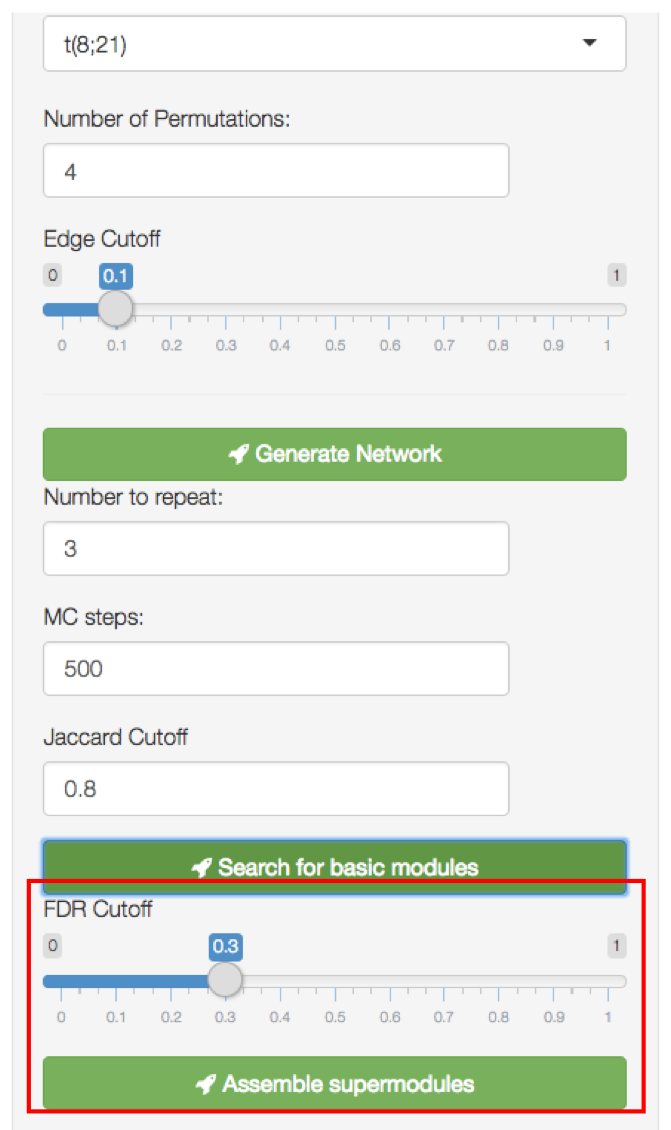
\includegraphics[scale=0.5]{./figure/MetaNetwork/MetaNetworkstep3}
\caption{MetaNetwork control panel for assemble supermodules step}
\label{fig:MetaNetworkstep3}
\end{center}
\end{figure}



\end{steps}

\subsubsection{Results}

We used the leukemia data to demonstrate the MetaNetwork module.
After merging the three datasets by filtering out 80\% of genes by mean and 80\% by variance, 206 genes remained.
In this example we only compare two phenotypes: inv(16) and t(8;21).
Detailed descriptions of these studies can be found in Table~\ref{tab:realDataLeukemia}. 
In general, the MetaNetwork tool is time consuming for large datasets (for both network generation and search for basic modules steps).
We generally suggest users to carefully restrict the number of genes (e.g. less than a thousand) for a test run before implementing large gene set.
By default, all outputs and several interim RData files will be automatically saved to the folder named ``MetaNetwork" under the working directory specified in Section~\ref{sec:setting}.




After the  \textbf{Generate Network} step is done, 
no output will show up in the screen. Instead, a message box will show up indicating several Rdata files are saved in the MetaNetwork folder. 
After \textbf{Search for basic modules} step is done, the screen will show a table of basic modules higher correlated in case or control, 
as in Figure~\ref{fig:MetaNetworkBM}. 
After \textbf{Assemble supermodules} assembly is done, screen will show a table of supermodules (Figure~\ref{fig:MetaNetworksuper}). 
Users can also select basic modules to plot (Figure~\ref{fig:MetaNetworkBMplot}). 
Meanwhile several files will be saved in the folder MetaNetwork
Detailed explanation of all these intermediate files are described in Section~\ref{sec:completeList_MetaNetwork}.
Note that because the module searching procedure is a random process, users may not be able to repeat the exact same results each time.

\begin{figure}[H]
\begin{center}
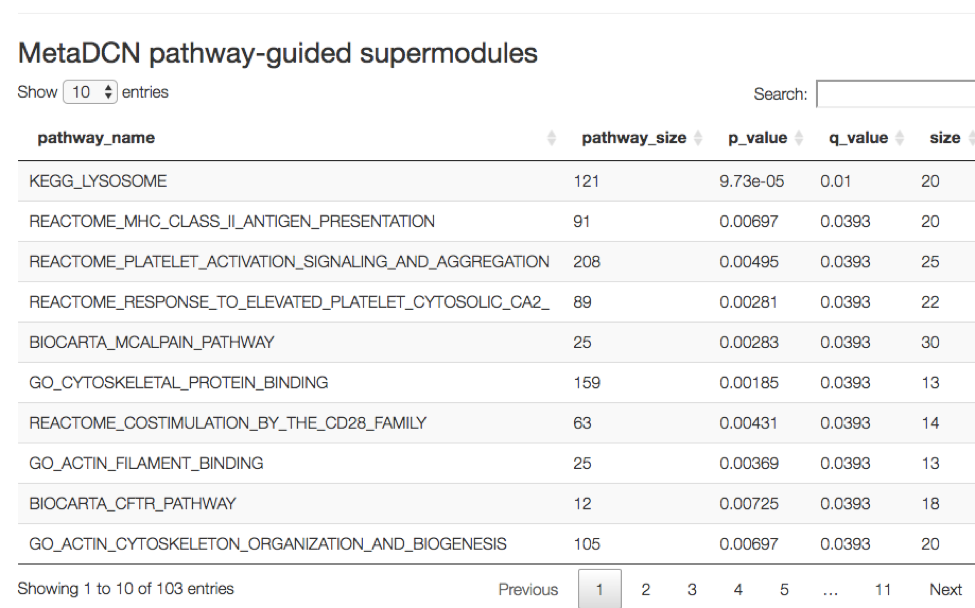
\includegraphics[scale=0.7]{./figure/MetaNetwork/MetaNetworksuper.png}
\caption{MetaNetwork supermodules table}
\label{fig:MetaNetworksuper}
\end{center}
\end{figure}

\begin{figure}[H]
\begin{center}
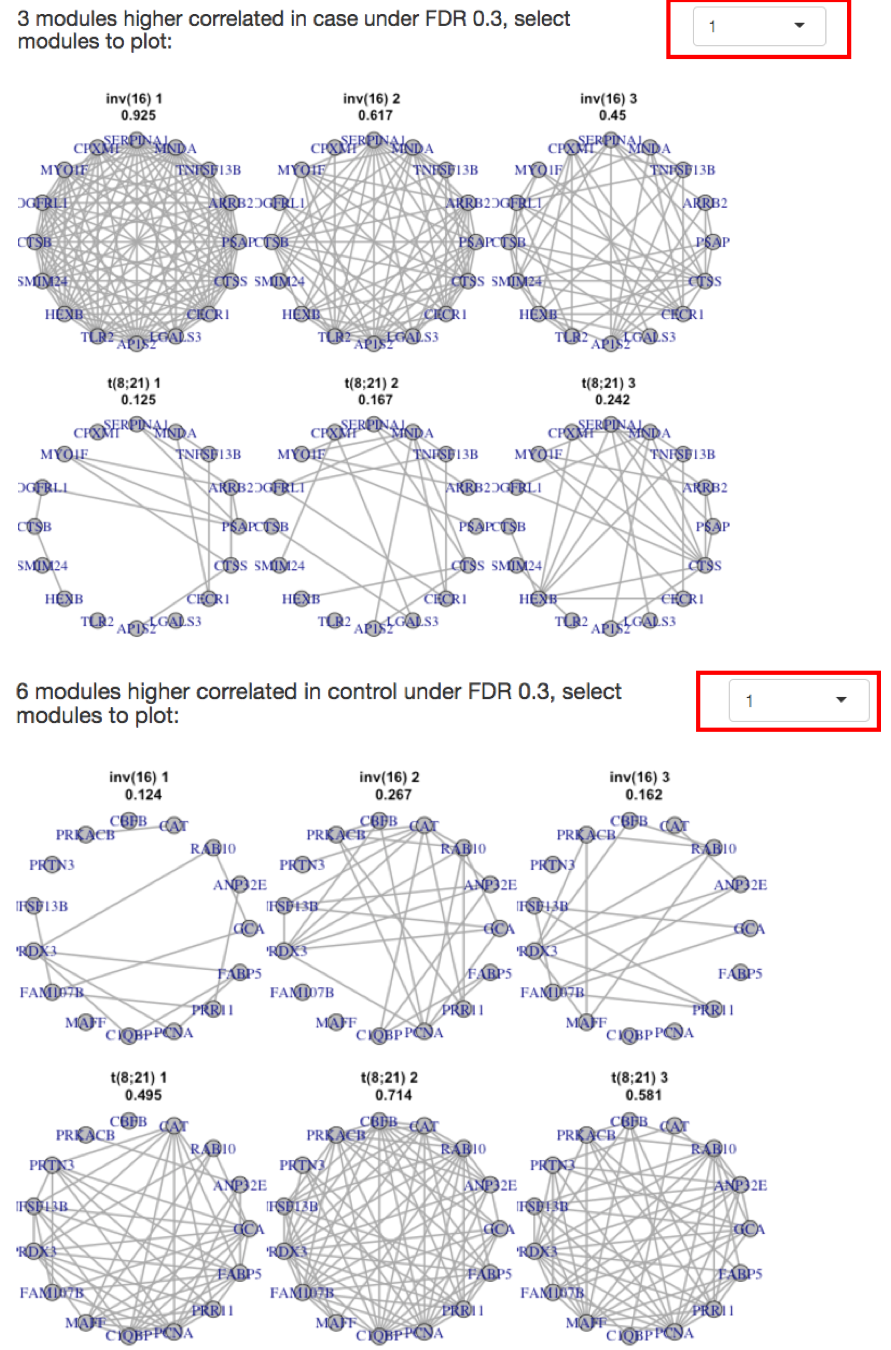
\includegraphics[scale=0.7]{./figure/MetaNetwork/MetaNetworkBMplot.png}
\caption{MetaNetwork select basic modules to plot.
Each dot represents a gene.
An edge represents the two genes are highly correlated.}
\label{fig:MetaNetworkBMplot}
\end{center}
\end{figure}
